\documentclass{article}
\usepackage{geometry}
\geometry{margin=0.8in}
\usepackage{natbib,hyperref}

\usepackage{doi}
\usepackage[utf8]{inputenc}
\usepackage{amsmath}
\usepackage{xcolor}

\usepackage{caption}
\usepackage{subcaption}
\usepackage{booktabs}
\newtheorem{theorem}{Theorem}
\title{Team 30 model}
\author{Jørgen S. Dokken and Igor A. Baratta}
\date{June 2021}

\newcommand{\curlp}[1]{\nabla \times \left(#1\right)}
\newcommand{\curl}[1]{\nabla \times #1}
\newcommand{\divmp}[1]{\nabla \cdot \left(#1\right)}
\newcommand{\divm}[1]{\nabla \cdot #1}

\newcommand{\mbf}[1]{\mathbf{#1}}
\newcommand{\ddn}[2]{\frac{\partial #1}{\partial #2}}
\newcommand{\dx}[0]{~\mathrm{d}x}
\newcommand{\ds}[0]{~\mathrm{d}s}
\newcommand{\dt}[0]{~\mathrm{d}t}

\newcommand{\pOmega}[0]{\partial\Omega}
\hypersetup{
    colorlinks=true,
    linkcolor=blue,
    filecolor=magenta,
    urlcolor=blue
    }
\usepackage{cleveref}
\usepackage{graphicx}

\usepackage{todonotes}
\newcommand{\igor}[1]{\todo[inline,color=blue!20, caption={2do}]{\textbf{Igor:}\\#1}}
\newcommand{\jorgen}[1]{\todo[inline,color=red!20, caption={2do}]{\textbf{J\o rgen:}\\#1}}

\usepackage{listings}
\RequirePackage{color}
\definecolor{pink}{RGB}{223,88,165}
\definecolor{deepgreen}{RGB}{100,146,82}
\definecolor{deepred}{RGB}{160,49,82}
\definecolor{lightyellow}{RGB}{255,253,233}
\RequirePackage{listings}
\lstdefinestyle{pythoncustom}
{
  language=Python,
  linewidth=\linewidth,
  basicstyle=\ttfamily\footnotesize,
  breaklines=true,
  otherkeywords={},             % Add keywords here
  keywordstyle=\color{pink},
  backgroundcolor=\color{lightyellow},
  commentstyle=\bfseries\color{deepgreen},    % Custom highlighting style
  stringstyle=\color{deepred},
  frame=single,                         % Any extra options here
  showstringspaces=false,
  numbers=left,
  tabsize=4
}

%-----------------------------------------------------------------------------
\begin{document}
%-----------------------------------------------------------------------------
\maketitle
%-----------------------------------------------------------------------------
\section{Governing laws and identities}

The classical electromagnetic field theory mainly describes and relates
four time-and space-dependent vector fields, current densities and
charge densities at any point in space and time
\cite{balanis2012advanced}. These quantities and their respective units
are presented in Table \ref{table:em_quantities}.
=
\begin{table}[!hb]
\centering
\caption{Electromagnetic Field Quantities}
\label{emquantities}
\begin{tabular}{|l|l|l|c|}
\cline{1-4}
      & Quantity & Unit & SI \\ \cline{1-4}
$ \mbf{E}(\textbf{x},t)$ & electric field intensity      & $V/m$ & $kg\cdot m\cdot s^{-3}\cdot A^{-1}$ \\
$ \mbf{H}(\textbf{x},t)$ & magnetic field intensity      & $A/m$ & $A\cdot m^{-1}$\\
$ \mbf{D}(\textbf{x},t)$ & electric flux density         & $C/m^2$ & $s \cdot A \cdot m^{-2}$   \\
$ \mbf{B}(\textbf{x},t)$ & magnetic flux density         & $Wb/m^2$ & $kg\cdot s^{-2}\cdot A^{-1}$   \\
$ \mbf{J}(\textbf{x},t)$ & electric current density         & $A/m^2$  & $A\cdot m^{-2}$  \\
$\textit{q}_e(\textbf{x},t)$ & electric charge density         & $C/m^3$ & $s\cdot A\cdot m^{-3}$    \\ \cline{1-4}
\end{tabular}
\label{table:em_quantities}
\end{table}

In its differential form, the set of Maxwell's equations can be written as follows
\begin{subequations}\label{eq:Maxwell}
    \begin{align}
    	\nabla \times \mbf{E} +  \frac{\partial \mbf{B}}{\partial t} &= 0, \label{faraday_simple}\\
    	\nabla \times \,  \mbf{H} +  \frac{\partial \mbf{D}}{\partial t} &=  \mbf{J}, \label{ampere_simple}\\
    	\nabla \cdot \,  \mbf{D} &= \textit{q}_{e}, \label{gaussE}\\
    	\nabla \cdot \,  \mbf{B} &= 0. \label{gaussM}
    \end{align}
\end{subequations}

Equation (\ref{faraday_simple}) is known as Faraday's Law, or law of
magnetic induction, and describes the effect of a changing magnetic
field on the electric field. Equation (\ref{ampere_simple}) is the
Ampère's circuital law generalized by Maxwell, which details how
electrical currents can generate a magnetic and changing electric fields
(displacement currents). Equation (\ref{gaussM}) states that the
magnetic field is a divergence-free or rotational field and Equation
(\ref{gaussE})  describes the relationship between the electric field
and the electric charges that cause it.

In most cases the constitutive equations refer to linear media and take
the following form:
\begin{subequations}
    \begin{align}
        \mathbf{B}&=\mu \mathbf{H} \\
        \mathbf{J}&=\sigma \mathbf{E}+\mathbf{J}_{0} \\
        \mathbf{D}&=\varepsilon \mathbf{E}
    \end{align}
\end{subequations}


\paragraph{Eddy Current Regime}
The Eddy Current model is obtained from the full set Maxwell equations
whenever the displacement current effects can be neglected

\begin{align}
    \frac{\partial \varepsilon \mathbf{E}}{\partial t} \ll \sigma E
\end{align}
which is always valid inside a passive metallic conductor provided the
time scale of interest is longer than the relaxation time of the
electric charge $t_r=\frac{\epsilon}{\sigma}$. The Maxwell's equations
inside a conductive domain $\Omega_c$ can then be approximated by
\begin{align}
    \left.
    \begin{array}{c}
        \nabla \times \mbf{H} = \mbf{J} \\
        \nabla \times \mbf{E} = -\frac{\partial \mbf{B}}{\partial t}\\
        \nabla \cdot \mbf{B}  = 0\\
        \nabla \cdot \mbf{J} = 0
    \end{array}
    \right\}
    \quad&\text{in } \Omega_c \label{eq:Maxwell:conductive}
\end{align}

For the non-conductive domain we adopt the magnetostatic approximation,
and the Maxwell's equations inside $\Omega_n$ can then be approximated
by

\begin{align}
    \left.
    \begin{array}{c}
        \nabla \times \mbf{H} = \mbf{J_0}\\
        \nabla \cdot \mbf{B} = 0
    \end{array}
    \right\}
    \quad&\text{in } \Omega_n \label{eq:Maxwell:nonconductive}
\end{align}

where $\mbf{H}$ is the magnetic field intensity, $\mbf{B}$ the magnetic
flux density, $\mbf{E}$ the electric field density, $\mbf{J}$ the Eddy
current density and $\mbf{J_0}$ the source term density.

\igor{Explain the continuity of electromagnetic fields.}
And the necessary continuity:
\begin{subequations}
    \begin{align}
        \mbf{B_n}  \cdot \mbf{n_n} + \mbf{B_c} \cdot \mbf{n_c} = 0   \quad&\text{on } \Gamma_{cn}\label{eq:cont} \\
        \mbf{H_n}  \times \mbf{n_n} + \mbf{H_c} \times \mbf{n_c} = 0   \quad&\text{on } \Gamma_{cn}
    \end{align}
\end{subequations}

The continuity conditions on the interface will provide the coupling
between the formulations in the nonconducting eddy current free region
$\Omega_n$ and the conducting eddy current region $\Omega_c$.

We have the following relations for the magnetic flux density $\mbf{B}$
and magnetic field intensity $\mbf{H}$

\begin{align*}
    \mbf{B}&=\begin{cases}
    \mu_0 \mbf{H} &\text{in air}\quad(\Omega_n)\\
    \mu_0 \mu_r \mbf{H} &\text{in magnetic linear material}\quad(\Omega_c).
    \end{cases}\\
    \mbf{J}&= \sigma \mbf{E} \text{ in } \Omega_c,
\end{align*}
which can be inverted to
\begin{subequations}
\begin{align}
    \mbf{H}&=\begin{cases}
        \nu_0 \mbf{B} &\text{in air}\quad(\Omega_n)\\
        \nu_0 \nu_R \mbf{B} & \text{in magnetic linear material}\quad(\Omega_c).
    \end{cases}\label{eq:HB}\\
    \mbf{E} &= \rho \mbf{J}\text{ in } \Omega_c.
\end{align}
\end{subequations}
where $\nu = \frac{1}{\mu}$, $\rho=\frac{1}{\sigma}$.
This means that we have the set of equations
\begin{subequations}
\begin{align}
    \left.\begin{array}{c}
        \curlp{\nu_0\nu_R \mbf{B}} = \mbf{J_0}\\
        \nabla \cdot \mbf{B} = 0
    \end{array}
    \right\}\quad&\text{in } \Omega_n \label{eq:Maxwell:n}\\
        \left.\begin{array}{c}
        \curlp{\nu_0\nu_R\mbf{B}} = \mbf{J} \\
        \curlp{\rho \mbf{J}} = -\frac{\partial \mbf{B}}{\partial t}\\
        \nabla \cdot \mbf{B}  = 0\\
        \nabla \cdot \mbf{J} = 0
    \end{array}
    \right\}\quad&\text{in } \Omega_c \label{eq:Maxwell:c}
\end{align}
\end{subequations}

%----------------------------------------A-phi formulation-----------------------------------
\section{A-V formulation}

\jorgen{We need some motivation here. I guess the issue is that we do
not have boundary conditions for $\mbf{B}$?} We use the vector calculus
identity for divergence of curl:

\begin{theorem}
    The divergence of \textit{any} vector field $\mbf{A}$ is always zero:
    \begin{align}
        \nabla \cdot (\nabla \times \mbf{A}) = 0.
    \end{align}
\end{theorem}
This identity can be used on $\divm{\mbf{B}}=0$ from
\cref{eq:Maxwell:c,eq:Maxwell:n} and therefore we define a vector
function $\mbf{A}$ such that
\begin{align}
    \mbf{B} = \curl{\mbf{A}}\label{eq:BA}.
\end{align}

Using the vector potential $\mbf{A}$, we combine the equations from
\cref{eq:Maxwell:conductive} and \cref{eq:Maxwell:c} to obtain
\begin{align*}
    \curl{\mbf{E}} &=\curlp{\rho \mbf{J}}= -\frac{\partial \mbf{B}}{\partial t}= -\curl{\frac{\partial \mbf{A}}{\partial t}}\\
    \curlp{\mbf{E}+\frac{\partial \mbf{A}}{\partial t}}&=0.
\end{align*}
We now use yet another vector calculus theorem
\begin{theorem}
    The curl of the gradient of any continuously twice-differentiable
    scalar field $\varphi$ always the zero vector:
    \begin{align}
        \nabla \times (\nabla \varphi)=0.
    \end{align}
\end{theorem}
In our case, we chose $V=-\phi$, and therefore
\begin{align*}
    0&=\curlp{\nabla\phi}=\curlp{-\nabla V}\\
    &=\curlp{\mbf{E}+\ddn{\mbf{A}}{t}}
\end{align*}
and therefore
\begin{align}
    \mbf{E}&=-\nabla V - \ddn{\mbf{A}}{t}.
\end{align}

We combine \cref{eq:HB} with \cref{eq:BA} and insert into \cref{eq:cont}
to obtain
\begin{align}
    \left.\begin{array}{r}
\mbf{n_c} \cdot \nabla \times \mbf{A_{c}}+\mbf{n_{n}} \cdot \nabla \times \mbf{A_n}=0 \\
\nu_{c} \nabla \times \mbf{A_{c}} \times \mbf{n_{n}}+\nu_{n} \nabla \times \mbf{A_{n}} \times \mbf{n_{n}}=\mbf{0}
\end{array}\right\} \text { on } \Gamma_{nc}. \label{eq:curl_grad}
\end{align}

To get our final set of equations, we insert the identity of $\mbf{E}$
into the $\divm{\mbf{J}}=0$. and obtain
\begin{subequations}
\begin{align}
    \curlp{\mu_R^{-1} \curl{\mbf{A}}} &= \mu_0\mbf{J_0}&&\text{in } \Omega_n\\
     \curlp{\mu_R^{-1} \curl{\mbf{A}}} + \mu_0\sigma\frac{\partial \mbf{A}}{\partial t} + \mu_0\sigma \nabla V &= \mbf{0} &&\text{in } \Omega_c\label{eq:strong2}\\
    \mu_0\divmp{\sigma \frac{\partial \mbf{A}}{\partial t} + \sigma \nabla V} &=0 &&\text{in } \Omega_c
\end{align}
\end{subequations}
Note that we have scaled the last equation by $\mu_0$ as it is a constant.

To ensure uniqueness of the magnetic vector potential, we use the gauge conditions
$\nabla \cdot \mbf{A}=0$.
This means that the third equation reduces to
\begin{align}
    \mu_0\divmp{ \sigma \nabla V} &=0&&\text{in } \Omega_c.
\end{align}
This gauge condition allows the usage of Lagrange elements.

%-----------------------------------------------------------------------------
\subsection{Frequency domain}

We assume that sources have only time-harmonic variation, so $\mbf{A}$
and $V$ can be written on the form $\mbf{A}=\hat{\mbf{A}} e^{+j\omega
t}$, $V= \hat{V} e^{+j\omega t}$ we can write the third equation as
\begin{align}
    \curlp{\mu_R^{-1} \curl{\hat{\mbf{A}}}} +j\omega \mu_0\sigma \hat{\mbf{A}} + \mu_0\sigma \nabla \hat{V} &= 0&&\quad \text{in } \Omega_n
\end{align}

%-----------------------------------------------------------------------------
\subsection{Weak formulation}

We introduce two function spaces, one space $\mathcal{V}$, a vector
space for our unknown $\mbf{A}$, and the space $\mathcal{Q}$ for our
scalar variable $V$. We multiply the first two equations by a test
function $\mbf{v} \in \mathcal{V}$ and integrate over the corresponding
domains. Then we end up with
\begin{align}
    \begin{split}
    &\int_{\Omega_n} \curlp{\mu_R^{-1} \nabla \times \mbf{A}} \cdot \mbf{v}\dx  + \int_{\Omega_c} \curlp{\mu_R^{-1} \nabla \times \mbf{A}}\cdot \mbf{v}\\
    &+ \mu_0\sigma \ddn{\mbf{A}}{t}\cdot \mbf{v} + \mu_0\sigma \nabla V \cdot \mbf{v}\dx
    =\int_{\Omega_n}\mu_0\mbf{J_0} \cdot \mbf{v} \dx
    \end{split}
\end{align}
We observe that the two first terms have a similar form, and we start by
considering the vector identity:
\begin{align*}
    (\curl{\mbf{D}})\cdot w&=  \divmp{\mbf{D} \times \mbf{w}} + \mbf{D}\cdot (\curl \mbf{w})
\end{align*}
Substituting $\mbf{D}=\mu_R^{-1}\curl \mbf{A}$ we get:
\begin{align*}
    (\curl{\mu_R^{-1}\curl\mbf{A}})\cdot w&=  \divmp{\mu_R^{-1}(\curl\mbf{A}) \times \mbf{w}} + \mu_R^{-1}(\curl\mbf{A})\cdot (\curl \mbf{w})
\end{align*}
Thus we have that
\begin{align}
    \int_{\Omega} \curlp{\mu_R^{-1} \nabla \times \mbf{A}} \cdot \mbf{v}\dx&=
    \int_{\Omega_n}\divmp{\mu_R^{-1}(\curl\mbf{A}) \times \mbf{v}} + \mu_R^{-1}(\curl\mbf{A})\cdot (\curl \mbf{v}) \dx
\end{align}
Using the divergence theorem (Gauss theorem) on the first term, we
obtain
\begin{align}
    \int_{\Omega} \curlp{\mu_R^{-1} \nabla \times \mbf{A}} \cdot \mbf{v}\dx&=
    \int_{\Omega}\mu_R^{-1}(\curl\mbf{A})\cdot (\curl \mbf{v}) \dx
    + \int_{\pOmega}\mu_R^{-1}\mbf{n}\cdot(\curl\mbf{A}) \times \mbf{v}\ds
\end{align}
For the boundary integral, we can use the identity:
\begin{align}
\begin{split}
    \mbf A\cdot (\mbf B\times \mbf C) = \mbf B\cdot(\mbf C \times \mbf A) = \mbf C \cdot (\mbf A \times \mbf B)\\
    \mbf n \cdot (\curl \mbf A \times \mbf v) = \mbf v \cdot (\mbf n \times \mbf \curl \mbf A)
\end{split}
\end{align}
Concluding, we write
\begin{align}
    \int_{\Omega} \curlp{\mu_R^{-1} \nabla \times \mbf{A}} \cdot \mbf{v}\dx&=
    \int_{\Omega}\mu_R^{-1}(\curl\mbf{A})\cdot (\curl \mbf{v}) \dx
    + \int_{\pOmega}\mu_R^{-1}\mbf{v}\cdot(\mbf{n}\times \curl\mbf{A})\ds
\end{align}
As we use this integration identity for the first term of both the first
and second integral, and observe that were $\Omega_c$ and $\Omega_n$
share a boundary, $\mbf{n}_c=-\mbf{n}_n$ and therefore the second
equation of \cref{eq:curl_grad} is satisfied as a natural boundary
condition, and we have:
\begin{align}
\begin{split}
    &\int_{\Omega_n\cup\Omega_c} \mu_R^{-1}(\curl\mbf{A})\cdot (\curl \mbf{v}) \dx
    + \int_{\pOmega}\mu_R^{-1}\mbf{v}\cdot(\mbf{n}\times \curl\mbf{A})\ds\\
    +& \int_{\Omega_c}\mu_0\sigma \ddn{\mbf{A}}{t}\cdot \mbf{v} + \mu_0\sigma \nabla V \cdot \mbf{v}\dx
    =\int_{\Omega_n}\mu_0\mbf{J_0} \cdot \mbf{v} \dx
\end{split}
\end{align}

Multiplying the third equation by a test function $-q\in \mathcal{Q}$
and integrate over $\Omega_c$ we obtain
\begin{align*}
    \int_{\Omega_c}-\mu_0\divmp{\sigma \nabla V} \cdot q &= 0 \qquad \forall q\in \mathcal{Q}_h
\end{align*}
We notice that this equation can be integrated by parts (and using that
we have the boundary condition $V=0$ on $\pOmega_c$ we obtain the
standard Poisson formulation Find $V^h\in\mathcal{Q}_{h,0}$ such that
\begin{align*}
    \int_{\Omega_c}\mu_0\sigma \nabla V \cdot \nabla q \dx &=0 \qquad \forall q\in \mathcal{Q}_h
\end{align*}
Combining the two sets of equations we have the following coupled system:
\begin{align}
\begin{split}
    &\int_{\Omega_n\cup\Omega_c} \mu_R^{-1}(\curl\mbf{A})\cdot (\curl \mbf{v}) \dx
    + \int_{\pOmega}\mu_R^{-1}\mbf{v}\cdot(\mbf{n}\times \curl\mbf{A})\ds\\
    +& \int_{\Omega_c}\mu_0\sigma \ddn{\mbf{A}}{t}\cdot \mbf{v} + \mu_0\sigma \nabla V \cdot \mbf{v}
    +\mu_0\sigma \nabla V \cdot \nabla q \dx
    =\int_{\Omega_n}\mu_0\mbf{J_0} \cdot \mbf{v} \dx
\end{split}
\end{align}

%-----------------------------------------------------------------------------
\subsection{Motion voltage term}

\igor{Add some motivation here}
We consider that the rotor moves with velocity $\mbf{u}$ relative to the
reference frame $\mathcal{O}(x,y)$ and a local reference frame
$\mathcal{O}'(x',y')$ which is moving with the rotor. Since low
frequencies are used in electrical machines displacement currents are
negligible. Therefore, the Maxwell equation can be written in the fixed
reference frame. The only change to the equations is that
$\mbf{E}'=\mbf{E}+\mbf{u}\times \mbf{B}$. We now have that
$\mbf{J}=\sigma\mbf{E}'=\sigma \mbf{E} + \sigma\mbf{u}\times \mbf{B}$.
For the other variables, we have that $\mbf{H}'=\mbf{H},
\mbf{B}'=\mbf{B}, \mbf{J}'=\mbf{J}$.

Using the $A-\phi$ formulation,
\begin{align*}
    \mbf{J}'=\mbf{J}=&=\sigma(-\ddn{\mbf{A}}{t}-\nabla V)=\sigma \mbf{E}\\
    \sigma\mbf{E}'&= \sigma(\mbf{E}+ \mbf{u}\times \mbf{B})\\
    \mbf{J}&= \sigma\left(-\ddn{\mbf{A}}{t}-\nabla V + \mbf{u} \times \mbf{B}\right)
\end{align*}
This means that \cref{eq:strong2} changes to:
\begin{align*}
     \curlp{\mu_R^{-1} \curl{\mbf{A}}} + \mu_0\sigma\frac{\partial \mbf{A}}{\partial t} + \mu_0\sigma \nabla V - \mu_0\sigma\mbf{u}\times(\curl{\mbf{A}}) &= \mbf{0} &&\text{in } \Omega_c
\end{align*}
This adds the following term:
\begin{align*}
    \int_{\Omega_c} -\mu_0\sigma \mbf{u} \times (\curl{\mbf{A}})\cdot \mbf{v} \dx
\end{align*}

%-----------------------------------------------------------------------------
\subsection{Special treatment of 2D problems}

As our input current $\mbf{J_0}=(0,0,J_{0})$, we get that
$\mbf{A}=(0,0,A_z)$ and we can solve a simple scalar equation for the
$z$ component of the magnetic potential. This means that we can write
$\curl{A}=\mbf{e}_x \ddn{A_z}{y}- \mbf{e}_y \ddn{A_z}{x}$

We can also assume that $\ddn{V}{z}=0$.
Thus we can simplify the terms in the weak formulation to:
\begin{subequations}
\begin{align}
    \int_{\Omega_n\cup\Omega_c}\mu_R^{-1}(\curl \mbf{A})\cdot(\curl \mbf{v})\dx & = \int_{\Omega_n\cup\Omega_n} \mu_R^{-1}\nabla A_z \cdot \nabla v_z \dx\\
    \int_{\pOmega}\mu_R^{-1} \mbf{v}\cdot (\mbf{n}\times\curl{\mbf{A}}) \ds &= \int_{\pOmega} \mu_R^{-1} v_z \left(n_x \ddn{A_z}{x} - n_y\ddn{A_z}{y}\right)\ds\\
    \int_{\Omega_c} \mu_0 \sigma \ddn{\mbf{A}}{t}\cdot \mbf{v} \dx &=
    \int_{\Omega_c} \mu_0 \sigma \ddn{A_z}{t}v_z \dx\\
    \int_{\Omega_c} \mu_0 \sigma \nabla V \cdot \mbf{v} \dx &=
    \int_{\Omega_c} \mu_0 \sigma \ddn{V}{z} v_x\dx = 0\\
    \int_{\Omega_c} \mu_0\sigma \nabla V \cdot \nabla q \dx &=
    \int_{\Omega_c} \mu_0\sigma \left(\ddn{V}{x}\ddn{q}{x} + \ddn{V}{y}\ddn{q}{y} \right)\dx\\
    \int_{\Omega_n} \mu_0 \mbf{J_0}\cdot \mbf{v} \dx &=
    \int_{\Omega_n} \mu_0 J_{0,z} v_z \dx
\end{align}
\end{subequations}

%-----------------------------------------------------------------------------
\subsubsection{Motion voltage term}
This adds the following term:
\begin{align*}
    \int_{\Omega_c} -\mu_0\sigma \mbf{u} \times (\curl{\mbf{A}})\cdot \mbf{v} \dx
    &=\int_{\Omega_c}\mu_0\sigma (\mbf{u}\cdot \nabla A_z)v_z \dx
\end{align*}
where $\mbf{u}=\omega_v(-r\sin(\theta), r\cos(\theta))=\omega_v(-y, x)$
and $r=\sqrt{x^2+y^2}, \theta = \arctan\left(\frac{y}{x}\right)$.

%-----------------------------------------------------------------------------
%----------------------EDGE elements--------------------------
\section{Comments about edge elements}

Note that in contrast to the similar formulation with nodal finite
elements, $A, V-A$ can be used even if the conductivity is
discontinuous.

The coupling of magnetic vector potential formulations in both regions
$$\left(A^{*}-A ; A, V-A ; A_{r}, V-A_{r}\right)$$ is straightforward.
The continuity of the tangential component of the vector potential on
$\Gamma_{n c}$ is explicitly satisfied through the use of the edge basis
functions. This enforces the continuity of $\boldsymbol{B} \cdot
\boldsymbol{n}$. The continuity of $\boldsymbol{H} \times
\boldsymbol{n}$ is accounted for in the weak sense by the surface
integrals of the form ... \cite{biro1999edge}.

With edge elements the interface are satisfied even in the presence of
discontinuities within domains.



%-----------------------------------------------------------------------------
\section{Derived quantities of interest}

%-----------------------------------------------------------------------------
\subsection{Maxwell's stress tensor}
We start by defining
\href{https://en.wikipedia.org/wiki/Maxwell_stress_tensor#Equation}{Maxwell's
stress tensor}
\begin{align*}
    \sigma_{ij} = \epsilon E_i E_j + \frac{1}{\mu_0} B_i B_j -\frac{1}{2}\left(\epsilon \mbf{E}\cdot \mbf{E} + \frac{1}{\mu_u}\mbf{B}\cdot \mbf{B} \right)\delta_{ij}
\end{align*}
where $\mbf{E}$ is the electric field, $\mbf{B}$ the magnetic flux
density and $\delta_{ij}$ the Kronecker-delta function. We would like to
compute the traction at a surface $\Gamma$ with normal $n$, i.e.
$d\mbf{F}=\mbf{n}\cdot\sigma=\sigma_{ij} n_i$, which can be written on
vector form as
\begin{align}
\begin{split}
     \mathrm{d} \mbf{F} &= \epsilon_0 (\mbf{n}\cdot\mbf{E}) \mbf{E} + (\mbf{n}\cdot \mbf{B}) \mbf{B} - \frac{1}{2} \left(\epsilon_0 \mbf{E}\cdot\mbf{E} + \frac{1}{\mu_0} \mbf{B} \cdot \mbf{B} \right)\mbf{n}\\
     &= \frac{1}{\mu_0}(\mbf{n}\cdot\mbf{B}) \mbf{B} - \frac{1}{2\mu_0}(\mbf{B}\cdot\mbf{B})\mbf{n}.
\end{split}
\end{align}
where the last equality comes from the fact that we are interested in
the stress tensor in the air surrounding the engine, where $\mbf{E}$ is
$\mbf{0}$.

%-----------------------------------------------------------------------------
\subsection{Electromagnetic torque}

The electromagnetic torque~\cite{reichert1976calculation} is obtained by
the integral
\begin{align}
    \mbf{T_e} &=L \int_\Gamma \left(\mbf{r} \times \mathrm{d} \mbf{F} \right)~\mathrm{d}\Gamma= L\int_{\Gamma} \frac{1}{\mu_0}(\mbf{B}\cdot\mbf{n})\mbf{r}\times\mbf{B}- \frac{1}{2\mu_0}(\mbf{B}\cdot\mbf{B})\mbf{r}\times\mbf{n}~\mathrm{d}\Gamma,
\end{align}
where $L$ is the depth of the domain and $\mbf{r}$ is the position
vector from the rotation axis to a point on the surface.

%-----------------------------------------------------------------------------
\subsubsection{Arkkio’s method}
It has been shown by Arkkio~\cite{Arkkio1987} that a volume formulation
of the torque is more stable than the surface integration when using
numerical approximations. The formulation used is:
\begin{align}
    \mathbf{T_e} = \frac{1}{\mu_0(r_o-r_i)}\int_{AirGap} rB_rB_\theta~\dx,
\end{align}
where $r_i$, $r_o$ is the inner and outer radius of the air gap, $B_r$
the radial component of the magnetic field, $B_\theta$ the azimuthal
direction, and $r=\vert \mbf{r}\vert$.

%-----------------------------------------------------------------------------
\subsubsection{2D simplification for surface torque}

In $2D$ as $\mbf{r}=(x,y,0)$, $\mbf{B}=(B_x, B_y), 0)$,
$\mbf{n}=(n_x,n_y,0)$ then
\begin{align}
    T_{e,z}&= L\int_{\Gamma} \frac{1}{\mu_0}(\mbf{B}\cdot\mbf{n})(r_x B_y - r_y B_x) - \frac{1}{2\mu_0}(\mbf{B}\cdot\mbf{B}(r_xn_y-r_yn_x) \mathrm{d}\Gamma
\end{align}
The boundary $\Gamma$ is a surface in the air-gap enclosing the rotor.

%-----------------------------------------------------------------------------
\subsection{Losses}

Applying an alternating magnetic field to a material, induces an
electromotiv force (emf) in the material, according to Faraday's law of
electromagnetic induction. The emf will circulate current within the
material, and these are called Eddy currents. The Eddy currents appear
due to a changes in the magnetic field. The currents are not responsible
for any useful work, and produces a loss in the material known as an
Eddy current loss (which in turn generates heat). Power dissipation is
given by
\begin{align*}
    P(t) = \int_{\Omega_{c}} \mbf{E'}\cdot \mbf{J'}\dx,
\end{align*}
where we have that $\mbf{J}'=\sigma\mbf{E}+ \mbf{u}\times \mbf{B}$, and we have
\begin{align}
    P(t) = \int_{\Omega_c}\sigma \mbf{E'}\cdot \mbf{E'}\dx,
\end{align}
In our examples, we will reach a periodic solution, and we are thus
interested in the power dissipation over a single period $t\in[T_0,
T_0+\frac{1}{\omega}]$
\begin{align}
    P_{period} = \int_{T_0}^{T_0+\frac{1}{\omega}} \int_{\Omega_c} \sigma \mbf{E'}\cdot \mbf{E'}\dx\dt
\end{align}
\igor{Add frequency domain formulation}

%-----------------------------------------------------------------------------
\subsection{Induced voltage}

The interlinkage flux $\boldsymbol{\phi}$ of the exciting coil can be
written as a function of the magnetic vector
potential~\cite{voltage2001}
\begin{align}
    \boldsymbol{\phi} = \frac{n_c}{S_c}\int_{\Omega_{coil}}\mbf{A}\cdot \mbf{n}_s \dx,
\end{align}
where $n_c, S_c$ is number of turns and cross sectional area of the
coil, $\mbf{n}_s$ a unit vector along the direction of the exciting
current. Note that we can decompose the exciting current as
\begin{align}
    \mbf{J}_0(t)= \frac{n_c}{S_c}I_0(t) \mbf{n}_s
\end{align}
and thus
\begin{align*}
    \boldsymbol{\phi} = \int_{\Omega_{coil}} \mbf{A}\cdot\mbf{J}_0/I_0\dx
\end{align*}
We have that the induced voltage $U$ is related to $\boldsymbol{\phi}$
as ~\cite{interlinkage2020}
\begin{align*}
    U=-\ddn{\boldsymbol{\phi}}{t}
\end{align*}
and therefore
\begin{align}
    U= \int_{\Omega_{coil}} -\ddn{\mbf{A}}{t}\cdot \mbf{n}_s\dx
\end{align}
We will compute the root mean squared value of the voltage over a period
in our examples. In other words, for each $U(t_i)=U_i, t_i=T_0+\Delta
t\cdot i, i \in [0, 1,\dots, \frac{\omega}{\Delta t}-1]$ we have
\begin{align}
    U_{RMS}=\sqrt{\frac{1}{\frac{\omega}{\Delta t}} \sum_{i=0}^{\omega/\Delta t -1}U_i^2}
\end{align}

\igor{Add frequency domain formulation}
%-----------------------------------------------------------------------------
\clearpage
\section{UFL formulation}

We use a backward Euler method to discretize $\ddn{A_z}{t}$, and the
variational form for  is written in UFL in \cref{code:ufl2D}
\begin{figure}[!ht]
    \centering
    \begin{lstlisting}[style=pythoncustom]
cell = triangle
coord_element = VectorElement("Lagrange", cell , 1)
mesh = Mesh(coord_element)
n = FacetNormal(mesh)
x = SpatialCoordinate(mesh)

FE = FiniteElement("Lagrange", cell, 1)
ME = MixedElement([FE, FE])
VQ = FunctionSpace(mesh, ME)

DG0 = FiniteElement("DG", cell, 0)
VDG = FunctionSpace(mesh, DG0)
dt = Constant(mesh)
mu_0 = 1.25663753e-6  # Permeability of air
mu_R = Coefficient(VDG)  # Relative permeability
sigma = Coefficient(VDG)  # Electrical conductivity
J0z= Coefficient(VDG)  # Current density
omega = Constant(mesh)

Az, V = TrialFunctions(VQ)
vz, q = TestFunctions(VQ)
AnVn = Coefficient(VQ)
An, Vn = split(AnVn) # Solution at previous time step

# Integration domains for single phase problem
# domains = {"Cu": (7, 8), "Stator": (6, ), "Rotor": (5, ), "Al": (4,), "AirGap": (2, 3), "Air": (1,)}

# Integration domains for three phase problem
domains = {"Cu": (7, 8, 9, 10, 11, 12), "Stator": (6, ), "Rotor": (5, ),
           "Al": (4,), "AirGap": (2, 3), "Air": (1,)}

# Create integration sets
Omega_n = domains["Cu"] + domains["Stator"] + domains["Air"] + domains["AirGap"]
Omega_c = domains["Rotor"] + domains["Al"]

# Define variational form
a = dt / mu_R * inner(grad(Az), grad(vz)) * dx(Omega_n + Omega_c)
a += dt / mu_R * vz * (n[0] * Az.dx(0) - n[1] * Az.dx(1)) * ds
a += mu_0 * sigma * Az * vz * dx(Omega_c)
a += dt * mu_0 * sigma * (V.dx(0) * q.dx(0) + V.dx(1) * q.dx(1)) * dx(Omega_c)
L = dt * mu_0 * J0z * vz * dx(Omega_n)
L += mu_0 * sigma * An * vz * dx(Omega_c)

# Motion voltage term
u = omega * as_vector((-x[1], x[0]))
a += dt * mu_0 * sigma * dot(u, grad(Az)) * vz * dx(Omega_c)

    \end{lstlisting}
    \caption{2D variational formulation for the $A-\phi$ problem}
    \label{code:ufl2D}
\end{figure}
\clearpage


%-----------------------------------------------------------------------------
\section{Team 30 benchmark}

The Team 30 model is a benchmark for
electromagnetics~\cite{daveyteam30}, where we have the following
computational domains:
\begin{figure}[!ht]
    \centering
    
\includegraphics[width=0.6\linewidth]{team_30_single_phase.png}
    \caption{Single phase model for TEAM 30}
    \label{fig:single_phase}
\end{figure}
\begin{figure}[!ht]
    \centering
    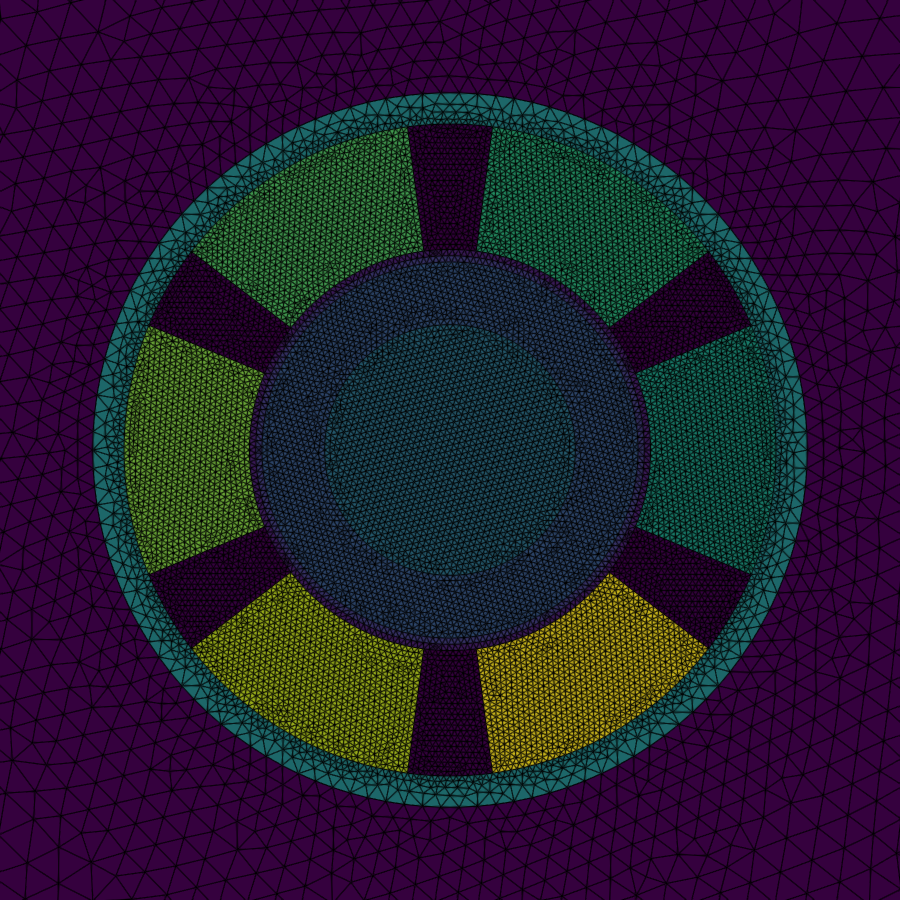
\includegraphics[width=0.6\linewidth]{team_30_three_phase.png}
    \caption{Three phase model for TEAM 30}
    \label{fig:three_phase}
\end{figure}
In both models there is an inner steel rotor (of radius $2$cm). The
steel rotor is encapsulated by an aluminum ring (inner radius $2$cm,
outer radius $3$cm). The ring with inner radius $3$cm and outer radius
$3.2$cm is filled with air. In the ring between $3.2$cm and $5.2$cm,
there are two alternating materials. The $45$ degree slices is copper (a
single winding) were current is induced. The other materials in this
ring is air. The final ring is laminated strator steel ($5.2$cm to
$5.7$cm), and the surrounding area is air.

Considering our equations from the prior sections, we have that
\begin{align}
    \Omega_c &= \Omega_{\text{rotor, steel}}\cup \Omega_{\text{rotor, alu}}\\
    \Omega_n &= \Omega_{\text{air}}\cup \Omega_{copper}\cup \Omega_{strator, steel}
\end{align}
For each of the domains we have the following material parameters
\begin{table}[!ht]
    \centering
    \begin{tabular}{|c|c|c|c|c|c|}\hline
         &  $\Omega_{\text{rotor, steel}}$ &  $\Omega_{\text{rotor, alu}}$ & $\Omega_{\text{air}}$ & $\Omega_{\text{copper}}$ & $\Omega_{\text{strator, steel}}$ \\\hline
        $\mu_0$ [H/m] &   $1.257\cdot 10^{-6}$ & $1.257\cdot 10^{-6}$ & $1.257\cdot 10^{-6}$ & $1.257\cdot 10^{-6}$ &  $1.257\cdot 10^{-6}$\\\hline
        $\mu_r$ & 30 & 1 & 1 & 1 & 30 \\\hline
        $\sigma [\Omega/m]$  & $1.6\cdot10^6$ & $3.72\cdot10^7$ & - & - &0 \\\hline
    \end{tabular}
    \caption{Material parameters of the TEAM 30 models}
    \label{tab:mat_params}
\end{table}

In each copper winding we have a current density $J=3.1\cdot 10^6 A/m^2$.
We can write $\mbf{J_0}(t)=(0,0,\alpha J\cos(\omega t + \beta))$ where the segment with center at angle $\theta$ has the following parameters
\begin{table}[!ht]
    \centering
    \begin{tabular}{|c|c|c|}\hline
    $\theta$& $\alpha$ & $\beta$  \\\hline
    0 & 1 & 0  \\\hline
    $\pi$ & -1 & 0 \\\hline
    \end{tabular}
    \caption{Single phase: Parameters for current.}
    \label{tab:single}
\end{table}

\begin{table}[!ht]
    \centering
    \begin{tabular}{|c|c|c|}\hline
    $\theta$& $\alpha$ & $\beta$  \\\hline
    0 & 1 & 0  \\\hline
    $\frac{\pi}{3}$ & -1 & $\frac{2\pi}{3}$ \\\hline
    $\frac{2\pi}{3}$ & 1 & $\frac{4\pi}{3}$ \\\hline
    $\pi$ & -1 & 0\\\hline
    $\frac{4\pi}{3}$ & 1 & $\frac{2\pi}{3}$ \\\hline
    $\frac{5\pi}{3}$ & -1 & $\frac{4\pi}{3}$\\\hline
    \end{tabular}
    \caption{Three phase: Parameters for current.}
    \label{tab:three}
\end{table}

For post-processing, the depth of the domain, $L$ is set to $1$m.

%-----------------------------------------------------------------------------
\subsection{Numerical results}

The variational formulation and domains have been implemented at
\href{https://github.com/Wells-Group/TEAM30/}{Github
Wells-Group/TEAM30}, and we do a numerical comparison of the derived
quantities listed in~\cite{daveyteam30}.

%-----------------------------------------------------------------------------
\subsubsection{Single phase engine}

We start by considering the single phase engine, which we solved in the
time domain, over $6$ phases, with 720 time steps per phase. The command
for running the study over the same rotational speeds as
in~\cite{daveyteam30} is shown below
\begin{lstlisting}[style=pythoncustom, numbers=none]
mpirun -n 5 python3 parametric_study.py --single --num_phases=6 --steps=720 --outdir=results_single_720
\end{lstlisting}

Following we have the computed quantities compared with those of the
benchmark for power dissipation, torque and induced voltage
\begin{table}[!ht]
\centering
\caption{Torque for single phase engine at various speeds. CG function space of degree 1 on mesh with 32626 elements}
\label{tab:torque:single}
\begin{tabular}{cccccc}
\toprule
$\omega$ & TEAM 30 &  Torque & Torque (Arkkio) & Relative Err & Relative Err (Arkkio) \\
\midrule
    0.00 &  0.0000 & -0.0056 &         -0.0000 &          inf &                   inf \\
   39.79 &  0.0528 &  0.0432 &          0.0485 &   1.8043e-01 &            8.0632e-02 \\
   79.59 &  0.0961 &  0.0971 &          0.0946 &   9.7400e-03 &            1.5987e-02 \\
  119.38 &  0.1431 &  0.1396 &          0.1408 &   2.3890e-02 &            1.5493e-02 \\
  159.17 &  0.1996 &  0.1929 &          0.1961 &   3.3299e-02 &            1.7331e-02 \\
  198.97 &  0.2754 &  0.2639 &          0.2698 &   4.1711e-02 &            2.0213e-02 \\
  238.76 &  0.3680 &  0.3523 &          0.3583 &   4.2596e-02 &            2.6216e-02 \\
  278.55 &  0.4421 &  0.4188 &          0.4261 &   5.2686e-02 &            3.6376e-02 \\
  318.35 &  0.3755 &  0.3472 &          0.3532 &   7.5349e-02 &            5.9289e-02 \\
  358.14 & -0.0707 & -0.0876 &         -0.0843 &   2.3888e-01 &            1.9170e-01 \\
\bottomrule
\end{tabular}
\end{table}


\begin{table}[!ht]
\centering
\caption{Loss for single phase engine at various speeds. CG function space of degree 1 on mesh with 32626 elements}
\label{tab:loss:single}
\begin{tabular}{ccccccc}
\toprule
$\omega$ & TEAM 30 (rotor) & Loss (rotor) & Relative Err (rotor) & TEAM 30 (steel) & Loss (steel) & Relative Err (steel) \\
\midrule
    0.00 &          341.77 &       341.18 &           1.7116e-03 &            3.94 &         3.92 &           6.0986e-03 \\
   39.79 &          341.25 &       340.76 &           1.4193e-03 &            3.93 &         3.91 &           6.1647e-03 \\
   79.59 &          340.46 &       339.90 &           1.6501e-03 &            3.90 &         3.88 &           6.2861e-03 \\
  119.38 &          340.04 &       339.45 &           1.7341e-03 &            3.85 &         3.82 &           6.6133e-03 \\
  159.17 &          340.23 &       339.55 &           1.9719e-03 &            3.77 &         3.74 &           7.1135e-03 \\
  198.97 &          339.30 &       338.50 &           2.3531e-03 &            3.64 &         3.61 &           8.0755e-03 \\
  238.76 &          333.62 &       332.67 &           2.8462e-03 &            3.40 &         3.37 &           9.2333e-03 \\
  278.55 &          317.99 &       316.96 &           3.2469e-03 &            3.00 &         2.97 &           1.0985e-02 \\
  318.35 &          288.08 &       287.57 &           1.7793e-03 &            2.36 &         2.33 &           1.0008e-02 \\
  358.14 &          256.64 &       257.44 &           3.0929e-03 &            1.67 &         1.67 &           2.0417e-03 \\
\bottomrule
\end{tabular}
\end{table}

\begin{table}[!ht]
\centering
\caption{Induced voltage (Phase A) for single phase engine at various speeds. CG function space of degree 1 on mesh with 32626 elements}
\label{tab:voltage:single}
\begin{tabular}{ccccccc}
\toprule
$\omega$ & TEAM 30 & Induced Voltage & Relative Error \\
\midrule
    0.00 &  0.5361 &          0.5359 &     3.4636e-04 \\
   39.79 &  0.5375 &          0.5372 &     4.5825e-04 \\
   79.59 &  0.5415 &          0.5413 &     4.2436e-04 \\
  119.38 &  0.5486 &          0.5484 &     3.8305e-04 \\
  159.17 &  0.5601 &          0.5599 &     3.7101e-04 \\
  198.97 &  0.5788 &          0.5786 &     4.3068e-04 \\
  238.76 &  0.6096 &          0.6091 &     9.3017e-04 \\
  278.55 &  0.6590 &          0.6575 &     2.1511e-03 \\
  318.35 &  0.7286 &          0.7248 &     5.0964e-03 \\
  358.14 &  0.7901 &          0.7833 &     8.5094e-03 \\
\bottomrule
\end{tabular}
\end{table}
% \begin{figure}[!ht]
%     \centering
%     \includegraphics[width=\linewidth]{rotor_loss_single_720.png}
%         \caption{Total rotor loss}
% \end{figure}
% \begin{figure}[!ht]
%          \centering
%         \includegraphics[width=\linewidth]{steel_loss_single_720.png}
%         \caption{Loss in steel}
% \end{figure}
% \begin{figure}[!ht]
%     \centering
%     \includegraphics[width=\linewidth]{torque_single_720.png}
%     \caption{Electromagnetic torque}
% \end{figure}
% \begin{figure}[!ht]
%      \centering
%     \includegraphics[width=\linewidth]{voltage_single_720.png}
%     \caption{Induced Voltage}
% \end{figure}

We observe that all derived quantities are within reasonable tolerance
from the reference data. We note, as described in the initial
data~\cite{daveyteam30}, that we have some trouble in approximating the
torque for the single phase engine. We also note that Arkkio's method
has a better approximation of the torque than the surface computation.

%-----------------------------------------------------------------------------
\subsubsection{Three phase engine}

Similarly, we do the same simulation for the three phase engine:
\begin{lstlisting}[style=pythoncustom, numbers=none]
mpirun -n 5 python3 parametric_study.py --num_phases=6 --steps=720 --outdir=results_three_720
\end{lstlisting}
We first consider the approximate torque, using surface integration and
Arkkio's method, as shown in \cref{tab:torque:three}
\begin{table}[!ht]
\centering
\caption{Torque for three phase engine at various speeds. CG function space of degree 1 on mesh with 32928 elements}
\label{tab:torque:three}
\begin{tabular}{cccccc}
\toprule
$\omega$ & TEAM 30 &  Torque & Torque (Arkkio) & Relative Err & Relative Err (Arkkio) \\
\midrule
       0 &  3.8259 &  3.7680 &          3.8153 &   1.5111e-02 &            2.7600e-03 \\
     200 &  6.5050 &  6.3581 &          6.4472 &   2.2588e-02 &            8.8948e-03 \\
     400 & -3.8926 & -3.7265 &         -3.7493 &   4.2691e-02 &            3.6830e-02 \\
     600 & -5.7594 & -5.6529 &         -5.7226 &   1.8493e-02 &            6.3888e-03 \\
     800 & -3.5908 & -3.5452 &         -3.5820 &   1.2699e-02 &            2.4302e-03 \\
    1000 & -2.7005 & -2.6689 &         -2.6967 &   1.1719e-02 &            1.4236e-03 \\
    1200 & -2.2500 & -2.2247 &         -2.2478 &   1.1243e-02 &            9.4123e-04 \\
\bottomrule
\end{tabular}
\end{table}


\begin{table}[!ht]
\centering
\caption{Loss for three phase engine at various speeds. CG function space of degree 1 on mesh with 32928 elements}
\label{tab:loss:three}
\begin{tabular}{ccccccc}
\toprule
$\omega$ & TEAM 30 (rotor) & Loss (rotor) & Relative Err (rotor) & TEAM 30 (steel) & Loss (steel) & Relative Err (steel) \\
\midrule
       0 &         1455.64 &      1453.09 &           1.7574e-03 &           17.41 &        17.30 &           6.1013e-03 \\
     200 &         1179.54 &      1171.55 &           6.7769e-03 &           16.99 &        16.76 &           1.3282e-02 \\
     400 &          120.01 &       121.82 &           1.5126e-02 &            1.38 &         1.33 &           3.6728e-02 \\
     600 &         1314.61 &      1315.53 &           6.9619e-04 &           17.88 &        17.74 &           7.3340e-03 \\
     800 &         1548.24 &      1558.85 &           6.8512e-03 &           16.89 &        16.90 &           6.6778e-04 \\
    1000 &         1710.69 &      1730.13 &           1.1368e-02 &           14.32 &        14.41 &           6.1830e-03 \\
    1200 &         1878.93 &      1909.49 &           1.6265e-02 &           12.01 &        12.15 &           1.1547e-02 \\
\bottomrule
\end{tabular}
\end{table}

\begin{table}[!ht]
\centering
\caption{Induced voltage (Phase A) for three phase engine at various speeds. CG function space of degree 1 on mesh with 32928 elements}
\label{tab:voltage:three}
\begin{tabular}{ccccccc}
\toprule
$\omega$ & TEAM 30 & Induced Voltage & Relative Error \\
\midrule
       0 &  0.6372 &          0.6370 &     2.5456e-04 \\
     200 &  0.8454 &          0.8448 &     6.6169e-04 \\
     400 &  1.4780 &          1.4595 &     1.2491e-02 \\
     600 &  0.7618 &          0.7616 &     2.4138e-04 \\
     800 &  0.6179 &          0.6176 &     5.2400e-04 \\
    1000 &  0.5757 &          0.5752 &     8.8976e-04 \\
    1200 &  0.5562 &          0.5556 &     1.0886e-03 \\
\bottomrule
\end{tabular}
\end{table}


We observe good correspondence between the compute quantities and the
reference data.
% \begin{figure}[!ht]
%     \centering
%     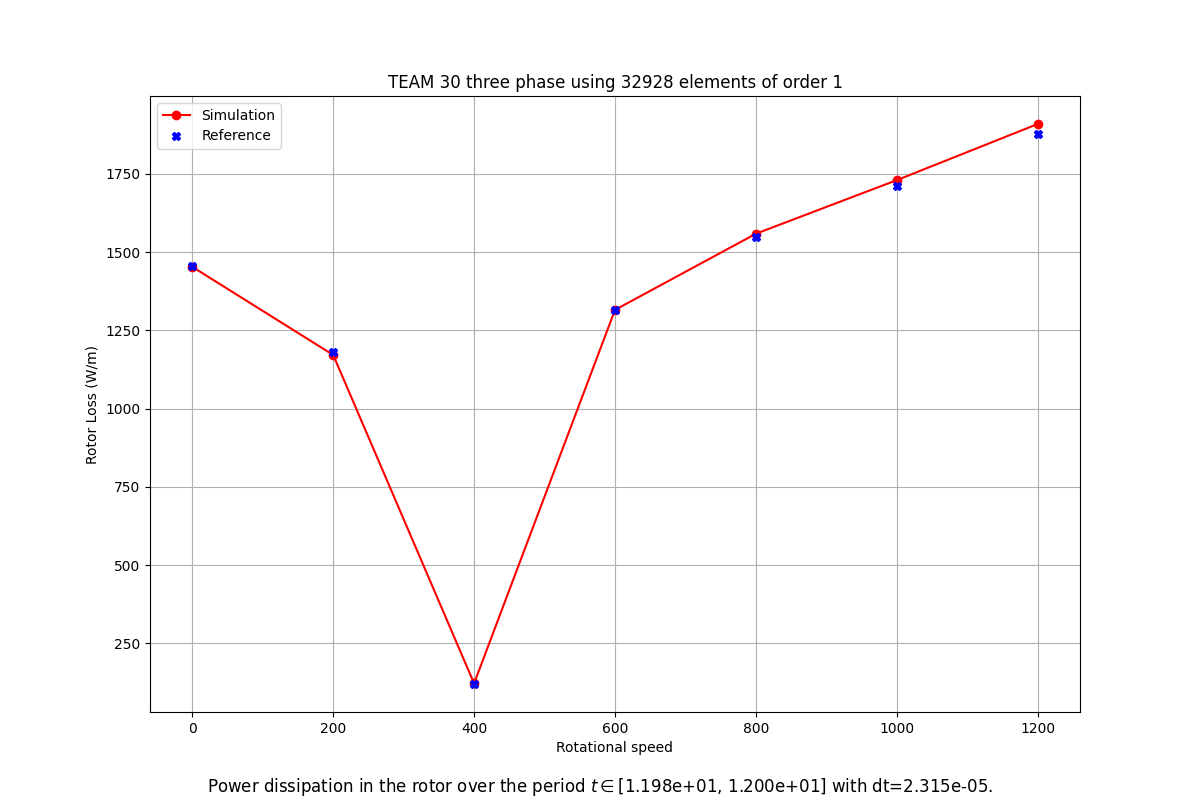
\includegraphics[width=\linewidth]{rotor_loss_three_720.png}
%         \caption{Total rotor loss}
% \end{figure}
% \begin{figure}[!ht]
%          \centering
%         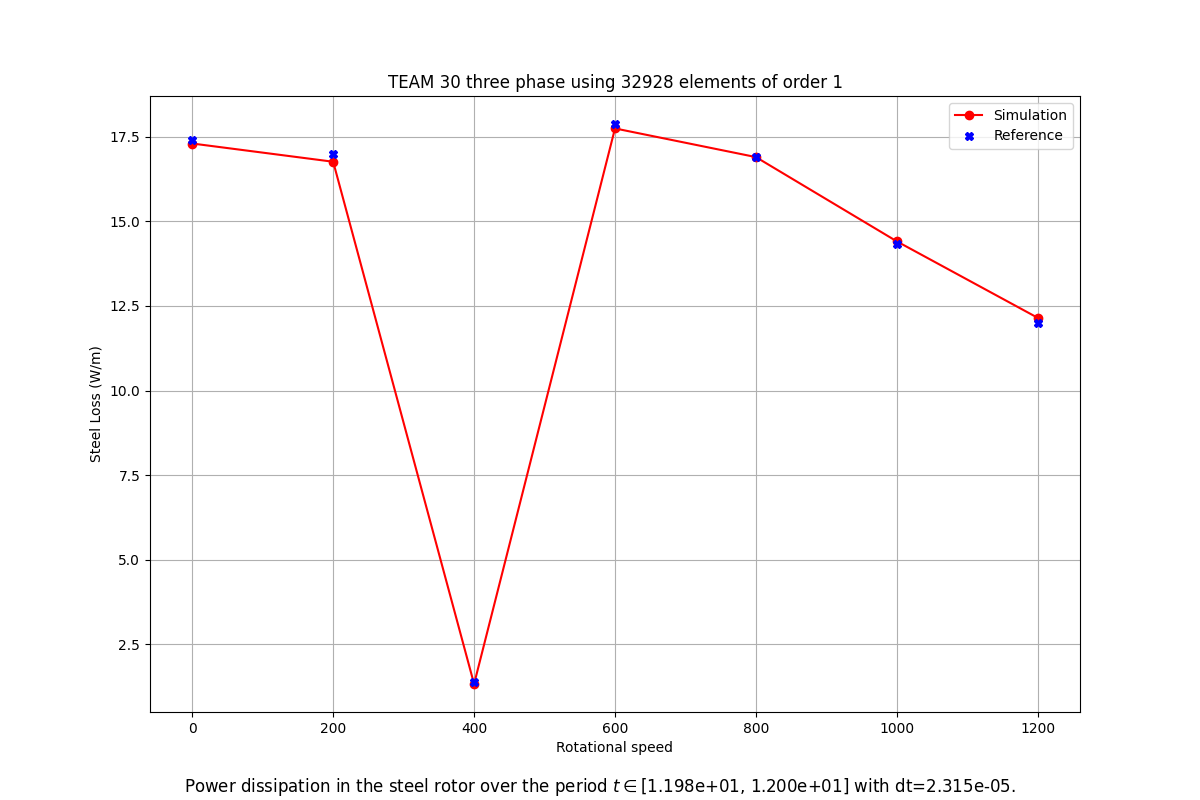
\includegraphics[width=\linewidth]{steel_loss_three_720.png}
%         \caption{Loss in steel}
% \end{figure}
% \begin{figure}[!ht]
%     \centering
%     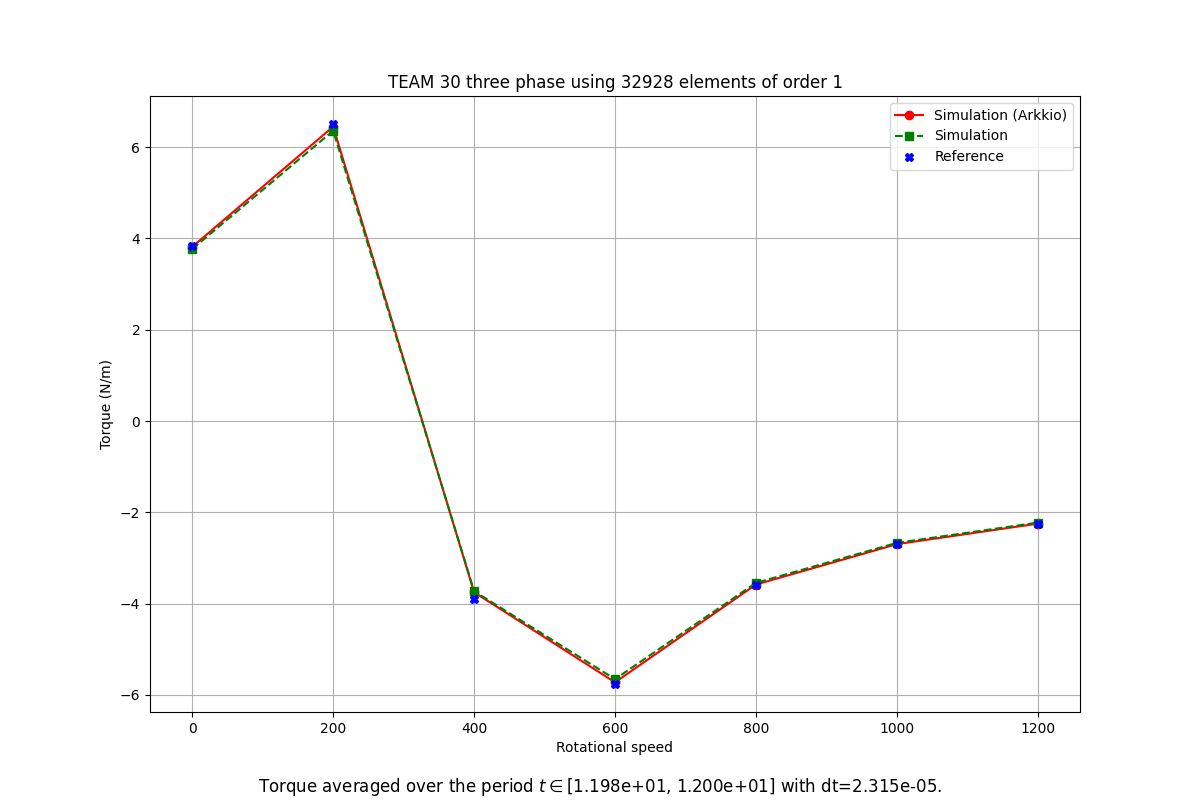
\includegraphics[width=\linewidth]{torque_three_720.png}
%     \caption{Electromagnetic torque}
% \end{figure}
% \begin{figure}[!ht]
%      \centering
%     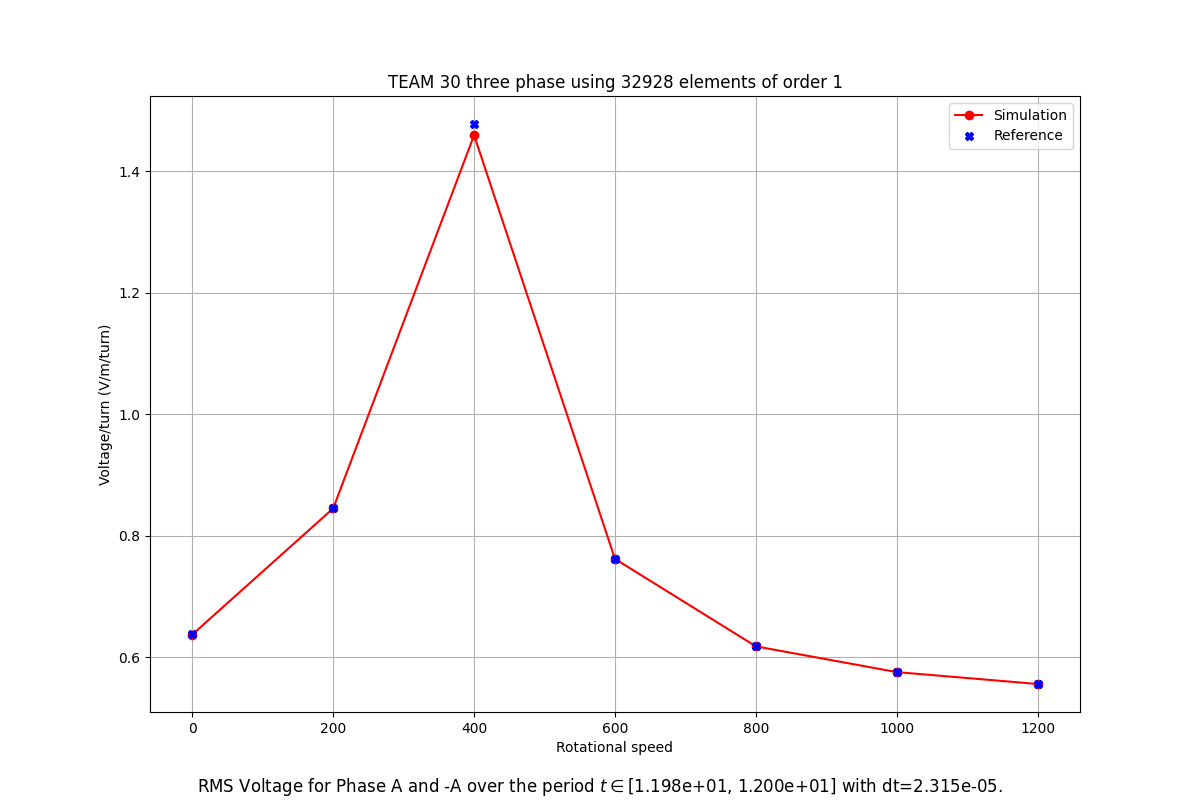
\includegraphics[width=\linewidth]{voltage_three_720.png}
%     \caption{Induced Voltage}
% \end{figure}

%-----------------------------------------------------------------------------
\bibliographystyle{plainnat}
\bibliography{references}
%-----------------------------------------------------------------------------
\end{document}
%-----------------------------------------------------------------------------
